\documentclass{article}
\usepackage[utf8]{inputenc}
\usepackage[english, science, small]{ku-frontpage}
\usepackage{tabularx}
\usepackage{indentfirst}
\usepackage{todonotes}
\usepackage{paralist}
\usepackage{fontawesome}
% higher rows in tables
\renewcommand{\arraystretch}{1.5}
\makeatletter
\renewcommand\tabularxcolumn[1]{>{\@minipagetrue}p{#1}}
\makeatother
\setdefaultleftmargin{1em}{}{}{}{}{}


\title{Software Engineering}
\subtitle{First hand-in}
\author{Matias Korn(crd551), Samuel Korn(rxq534), Nikolin Prenga (hpq143), Silvan Adrian (zlp432)}
\date{\today}

\begin{document}

\maketitle

% solution and problem domain
\section{Solution and problem domain}
Citizens have the possibility to apply for loss of earnings. Loss of earnings means, that the earnings the citizen has missed out on, due to being occupied of taking care of a child. There are many actors involved when the citizen apply for loss of earnings. First off, there is the case-worker, who receives the application from the citizen. The case-worker is working at a municipality council. The municipality council has to comply with the law and paragraph 42 and the rules that are provided from the ministry of social affairs.

\vspace{2mm}

The ministry of social affairs lay down the rules of:
(1) How big a possible cap of allowed compensation is.
(2) How much the pension scheme is obligated to contribute with. (3) How the calculation of the actual compensation is made. (4) What the limit is of how much the pension scheme is obligated to contribute with. (5) How much of the loss on the pension contribution shall be paid by the receiver and municipal council.

\vspace{2mm}

As mentioned, the case-workers handles the cases and receives all the necessary information, for complying with paragraph 42. First of, the case-worker has to establish, if there are grounds for compensation. (1) The child has to be under 18. (2) The conditions on the child's health have to abide by the law, for that the child's health record has to be collected from the health care system. The health record has to confirm, that it is most expedient for the mother or father to the care of the child, at home or has been placed in care under section 52(3)(vii). If that is the case, the condition is, that it is most expedient for a parent to be there. It might be difficult to establish, if that is the case, based on the health record, if it is not explicitly stated, therefore it might be necessary to collect a confirmation by the child's doctor. (3) Loss of income has to be established, for that the necessary bank statements have to be provided.

\vspace{2mm}

Our solution is concerned with case management. We have to provide a platform for collecting, recording the progress and the final decisions that have been made and what grounds there has been for them. The following actors are directly involved in our system: (1) the citizen, (2) the case-worker, (3) the ministry of social affairs(external system), (4) the law that decides if the citizen is permitted for loss of earnings, (5) the payment system(external system), that is available for the municipal council. Our solution will handle the information gathering and storing.

% scenarios
\newpage
\section{Scenarios}
\todo[inline]{Add an additional from the user/parent points of view not too focused on caseworker only}
\subsection*{Application approved}
\begin{table}[htb!]
\begin{tabularx}{\textwidth}{l|X}
	\textbf{Scenario name} & Application approved \\
	\hline
	\textbf{Participating actor instances} & Alice:applicant, Bob:caseworker\\
	\hline
	\textbf{Flow of events} &
	\begin{compactenum}
			\item Alice, a parent, has a child with a serious chronic illness. She logs into the OCM system as a citizen, fills out a form, attaches any relevant documentation and submits the application. There does not exist any prior applications from Alice, so the system annotates it as a new case.
			\item The system assigns the application to caseworker Bob. He logs into the system as a caseworker. He picks Alice's application from an overview of assigned cases. He validates documentation authenticity and data entered in form by Alice. He approves and submits the application.
			\item The system assigns the application to another caseworker Charles. He processes the application in the same manner as Bob and submits it once it is approved.
			\item With approvals from two random caseworkers, the system annotate the case as approved and calculates the compensation based on the data contained in the application. The system sends a response to Alice's e-mail that her application was approved, including the details regarding her compensation. The system archives the case.
    \end{compactenum}\\
	\hline
\end{tabularx}
\end{table}


\subsection*{Application rejected}
\begin{table}[htb!]
\begin{tabularx}{\textwidth}{l|X}
	\textbf{Scenario name} & Application rejected \\
	\hline
	\textbf{Participating actor instances} & Alice:applicant, Bob:caseworker, Charles:CaseWorker\\
	\hline
	\textbf{Flow of events} &
	\begin{compactenum}
	       \item Alice is a parent that has a child suffering from fever. She logs into the OCM system as a citizen, fills out the application form, attaches any relevant documentation and submits the application. There does not exist any prior applications from Alice, hence the system annotates it as a new case.
           \item  The system assigns the application to caseworker Bob. He logs into the system as a caseworker. He picks Alice's application from an overview of assigned cases. He validates documentation authenticity. The applicant is not eligible for compensation, so he rejects and submits the application.
           \item The system assigns the application to another caseworker Charles. He concludes the same as Bob. Charles also rejects and submits the application.
	        \item With rejections from two random caseworkers, the system annotate the case as rejected. The system sends a response to Alice's e-mail that her application was rejected. The system archives the case.
	\end{compactenum}\\
	\hline
\end{tabularx}
\end{table}

\newpage
\subsection*{Disputed application approval}
\begin{table}[htb!]
\begin{tabularx}{\textwidth}{l|X}
	\textbf{Scenario name} & Disputed application approval \\
	\hline
	\textbf{Participating actor instances} & Alice:applicant, Bob:caseworker, Charles:Caseworker\\
	\hline
	\textbf{Flow of events} &
	\begin{compactenum}
	        \item Alice, a parent, has a child with an ambiguous illness in the context of "loss of earnings" legislation. She logs into the OCM system as a citizen, fills out a form, attaches any relevant documentation and submits the application. There does not exist any prior applications from Alice, so the system annotates it as a new case.
	        \item The system assigns the application to caseworker Bob. He logs into the system as a caseworker. He picks Alice's application from an overview of assigned cases. He validates documentation authenticity and data entered in form by Alice. He approves and submits the application.
	        \item The system assigns the application to another caseworker Charles. He validates documentation authenticity and data entered in form by Alice. He rejects and submits the application.
	        \item With an approval and rejection, the system assigns the application to yet another caseworker Diana. She validates documentation authenticity and data entered in form by Alice. She approves and submits the application.
	        \item With approvals from two random caseworkers, the system annotate the case as approved and calculates the compensation based on the data contained in the application. The system sends a response to Alice's e-mail that her application was approved, including the details regarding her compensation. The system archives the case.
	   	\end{compactenum}\\
	\hline
\end{tabularx}
\end{table}

\newpage
\subsection*{Inquire additional information from applicant}
\begin{table}[htb!]
\begin{tabularx}{\textwidth}{l|X}
	\textbf{Scenario name} & Inquire additional information from applicant \\
	\hline
	\textbf{Participating actor instances} & Alice:applicant, Bob:caseworker, Charles:Caseworker\\
	\hline
	\textbf{Flow of events} &
	\begin{compactenum}
	        \item Alice, a parent, has a child with a serious chronic illness. She logs into the OCM system as a citizen, fills out a form inadequately and submits the application. There does not exist any prior applications from Alice, so the system annotates it as a new case.
	        \item The system assigns the application to caseworker Bob. He logs into the system as a caseworker. He picks Alice's application from an overview of assigned cases. The application is filled out inadequately, so he writes an e-mail to Alice and inquire about missing information. He sets the case on hold and waits for a response from applicant.
	        \item Alice fills out the missing data and submits the changes. 
	        \item Bob resumes its progress and approves the application and submit it to the system.
	        \item The system assigns the application to another caseworker Charles. The case now contains the additional information added by Bob. Charles validate the contained data, approves the application and submits it.
	        \item With approvals from two random caseworkers, the system annotate the case as approved and calculates the compensation based on the data contained in the application. The system sends a response to Alice's e-mail that her application was approved, including the details regarding her compensation. The system archives the case.
	\end{compactenum}\\
	\hline
\end{tabularx}
\end{table}

\newpage
\subsection*{Illegitimate application approval}
\begin{table}[htb!]
\begin{tabularx}{\textwidth}{l|X}
	\textbf{Scenario name} &  Illegitimate application approval\\
	\hline
	\textbf{Participating actor instances} & Alice:applicant, Bob:caseworker, Charles:Caseworker\\
	\hline
	\textbf{Flow of events} &
	\begin{compactenum}
	        \item Alice, a parent, has a child with a fever. She logs into the OCM system as a citizen, fills out a form, attaches any relevant documentation and submits the application. There does not exist any prior applications from Alice, so the system annotates it as a new case.
	        \item The system assigns the application to caseworker Bob. He logs into the system as a caseworker. He picks Alice's application from an overview of assigned cases. He approves without validating contents and submits the application.
            \item The system assigns the application to another caseworker Charles. He also approves the application without validating its contents and submits it.
            \item With approvals from two random caseworkers, the system annotate the case as approved and calculates the compensation based on the data contained in the application. The system sends a response to Alice's e-mail that her application was approved, including the details regarding her compensation. The system archives the case.
            \item this should not happen blah blah blah and what went wrong
	\end{compactenum}\\
	\hline
\end{tabularx}
\end{table}

\newpage
\subsection*{Duplicate application approved}
\begin{table}[htb!]
\begin{tabularx}{\textwidth}{l|X}
	\textbf{Scenario name} &  Duplicate application approved\\
	\hline
	\textbf{Participating actor instances} & Alice:applicant, Bob:caseworker, Charles:Caseworker\\
	\hline
	\textbf{Flow of events} &
    \begin{compactenum}
	        \item Alice, a parent, has forgot she already receives "loss of earnings" compensation for her child. She logs into the OCM system as a citizen and fills out a form, attaches any relevant documentation and submits the application. There exist prior applications from Alice, so the system annotates it as a duplicate case.
	        \item The system assigns the application to caseworker Bob. He logs into the system as a caseworker. He picks Alice's application from an overview of assigned cases. He approves without noticing this is a duplicate case and submits the application.
	        \item The system assigns the application to another caseworker Charles. He also approves the application without noticing this is a duplicate case and submits it.
	        \item With approvals from two random caseworkers, the system annotate the case as approved and calculates the compensation based on the data contained in the application. The system sends a response to Alice's e-mail that her application was approved, including the details regarding her compensation. The system archives the case.
    \end{compactenum}\\
	\hline
\end{tabularx}
\end{table}

% fuctional requirements
\newpage
\section{Functional requirements}

The system contains a login function for both caseworkers and applicants. Caseworkers login to the system through an employee portal, while applicants login to the system using NemId. The system validates eligible applicants through NemId.

\vspace{2mm}

Once the applicant is logged in, they are presented with a form through which they submit relevant information. The form contains text input fields and fields through which additional documentation can be attached to the case as pdf files.

\vspace{2mm}

The system assigns submitted cases to available caseworkers at random. Processed cases are archived and saved in an immutable state. Cases are annotated based on their state, i.e. ongoing, archived or on hold. Cases from the same citizen are also annotated in order to detect possible duplicates.

\vspace{2mm}

Once logged in, the caseworker is presented with their assigned cases, as well as a way to search all archived cases. More specifically, the caseworker cannot see ongoing cases not assigned to them, however all archived cases are search-able no matter the assigned caseworker. Caseworkers have access to all data submitted in the cases by the applicant. While processing a case, the caseworker can approve or reject cases. If the case is approved, the system calculates the "loss of earnings" benefits based on the data contained in the case and the current applicable laws. The system informs the applicant of the final decision, containing the benefits calculations if approved, through an e-mail.

\vspace{2mm}

A caseworker can set a case on hold if the documentation is insufficient. In such a case, the cases state must be changed to on hold and the system sends an e-mail to the applicant informing them of the cases state. The caseworker is able to write the message contained in the e-mail. The applicant is able to access the case form through a link in the e-mail, where the applicant can submit the missing information.
The caseworker can afterwords reprocess the case and either reject or approve the case.

\vspace{2mm}

In case the System annotated a case as a possible duplicate and the caseworker decides this to be true, then the case state must be changed to rejected.

\vspace{2mm}

A caseworker can be assigned a supervisor role, giving them additional functions. A supervisor is able to see all ongoing and archived cases, as well as which caseworkers has been assigned to which case and the cases current state.
\newpage
\begin{figure}[htb!]
	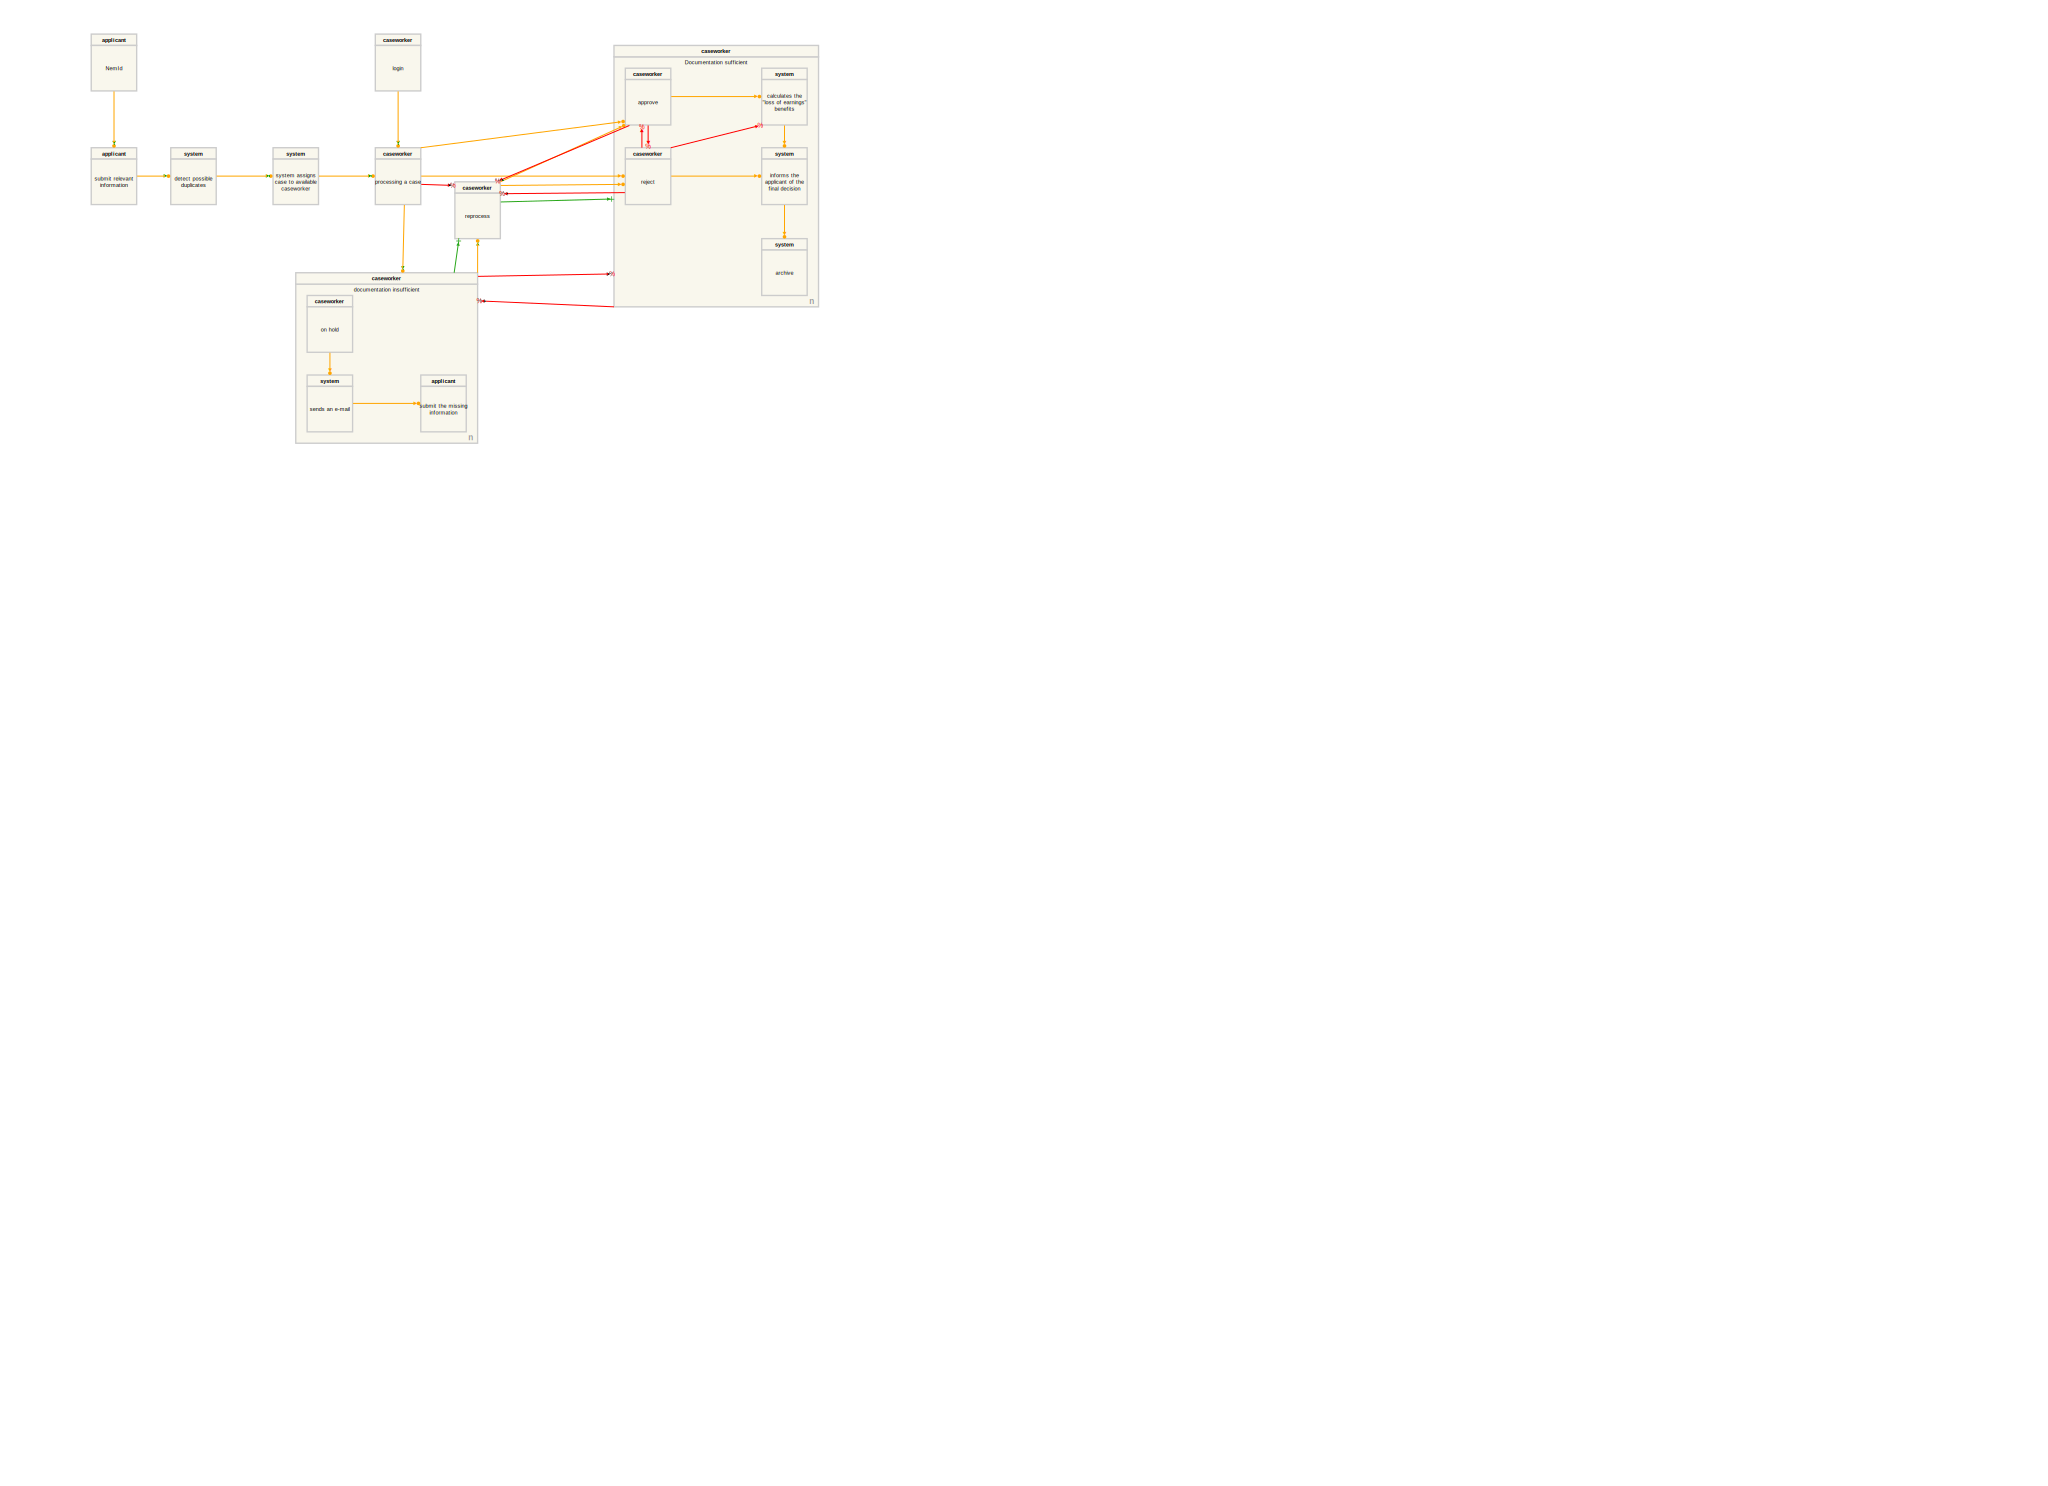
\includegraphics[]{dcrgraph/dcrgraph.svg}
	\caption{DCR graph}
\end{figure}

\newpage
\begin{figure}[htb!]
    \centering
    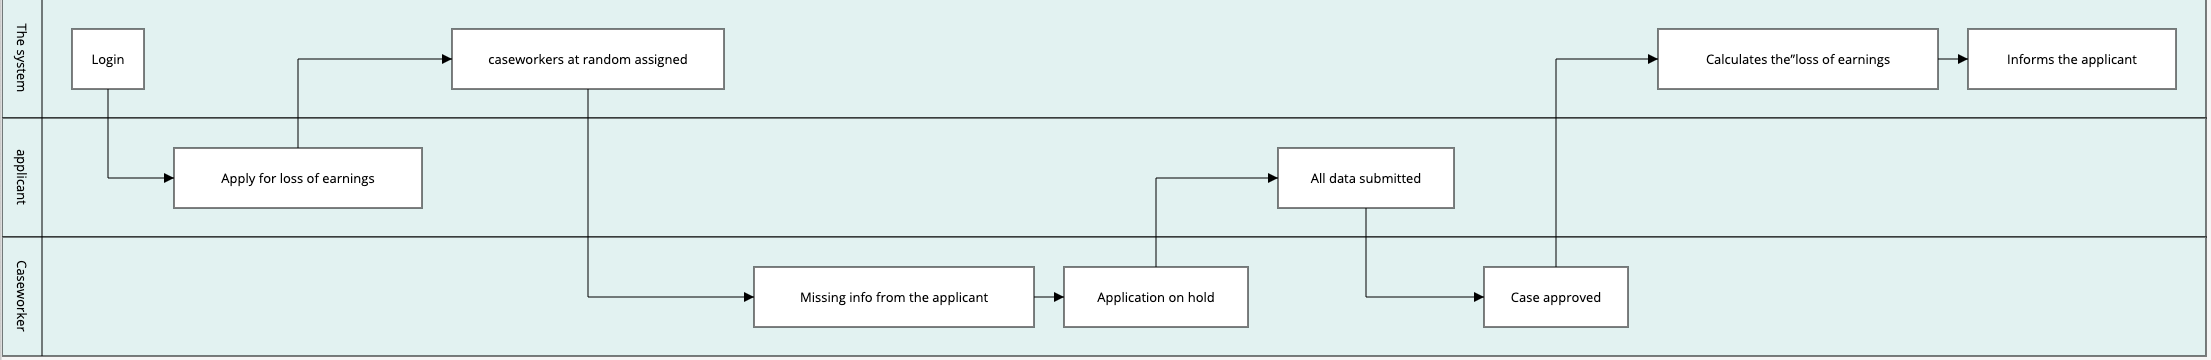
\includegraphics[width=\textwidth]{img/swim-case-approved.png}
    \caption{Case approved}
\end{figure}

\begin{figure}[htb!]
    \centering
    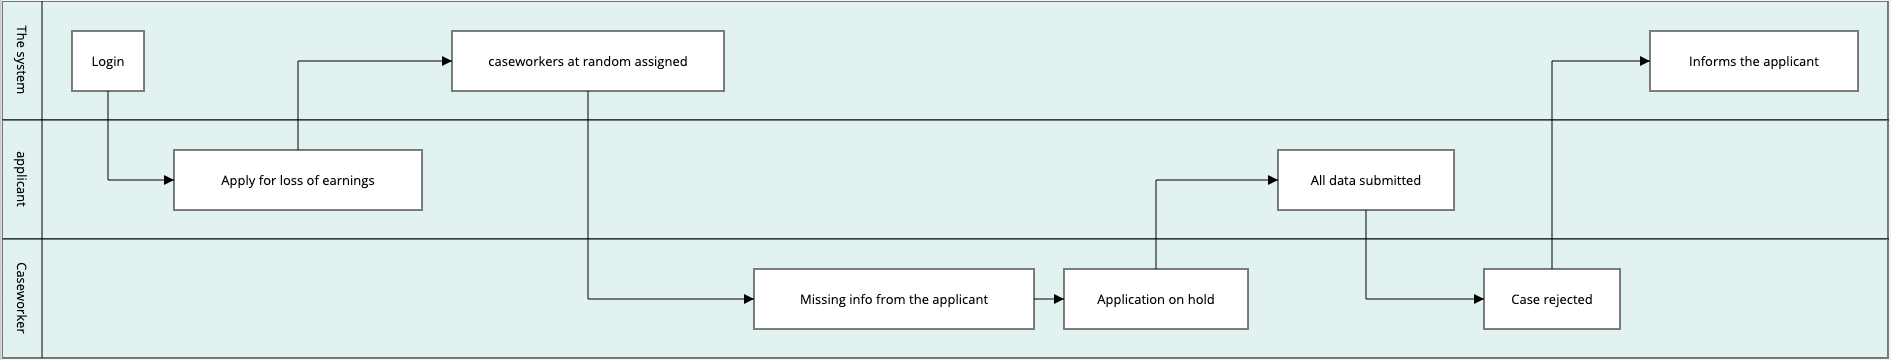
\includegraphics[width=\textwidth]{img/swim-case-rejected.png}
    \caption{Case rejected}
\end{figure}

\begin{figure}[htb!]
    \centering
    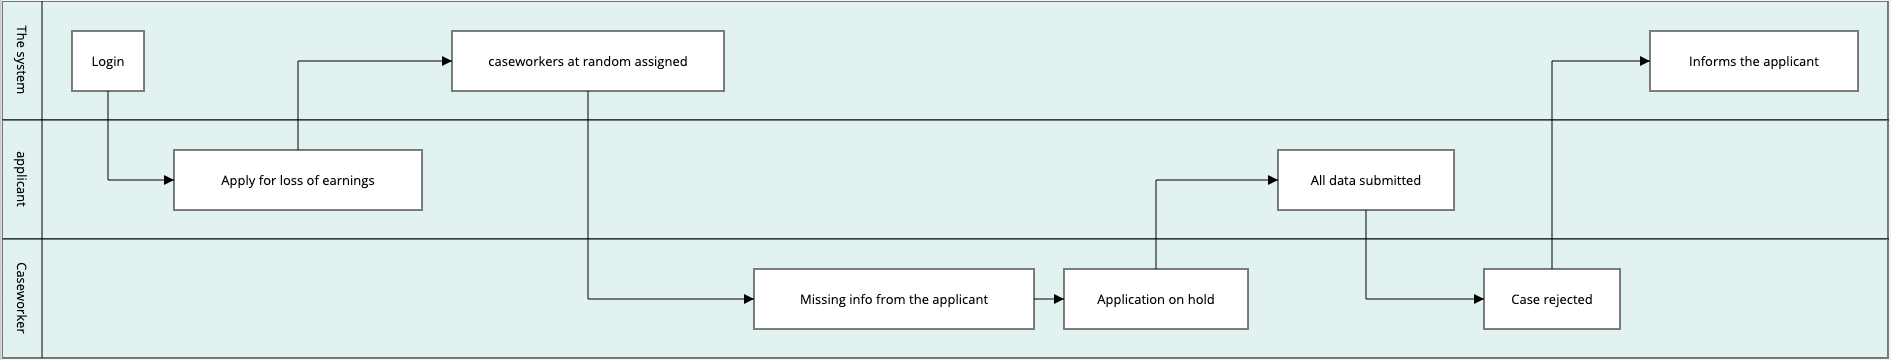
\includegraphics[width=\textwidth]{img/swim-case-rejected.png}
    \caption{Case inquire more information}
\end{figure}

%non functional requirements
\newpage
\section{Non-functional requirements}
\label{sec:nfr}
\begin{table}[htb!]
\begin{tabularx}{\textwidth}{l|X}
	\textbf{Category} & \textbf{Nonfucntional Requirements} \\
	\hline
	\textbf{Availability} & 
	    \begin{compactitem}
	        \item Tolerated application downtime is one hour a month.
	    \end{compactitem}\\
	\hline
	\textbf{Usability} &
	    \begin{compactitem}
	        \item People with no training should able to use the software and finish an application within 20 minutes.
	    \end{compactitem}\\
	\hline
	\textbf{Accessibility} & 
	\begin{compactitem}
	    \item The software should be accessible for people with disabilities by following the WCAG 2.1 standard.
	\end{compactitem}\\
	\hline
	\textbf{Maintainability} &
	    \begin{compactitem}
	        \item The cyclomatic complexity of code must not exceed 7.
	        \item Methods should not exceed 100 lines of code.
	        \item Installation of a new Version shall leave all database content and personal user settings unchanged.
	    \end{compactitem}\\
	\hline
	\textbf{Performance} &
	\begin{compactitem}
        \item Pages should be loaded in between 2-6 Seconds.
	\end{compactitem}\\
	\hline
	\textbf{Testability} &
	    \begin{compactitem}
	        \item The system should include unit tests that ensure line coverage of 80\%.
	        \item The system should include End to End tests to ensure all happy paths are covered.
	    \end{compactitem}\\
	\hline
	\textbf{Security} & 
		\begin{compactitem}
    	        \item The system needs to uphold the GDPR legislation.
    	        \item No one should have access on data he/she has no access rights on.
	    \end{compactitem}\\
	\hline
	\textbf{Scalability} & 
	    \begin{compactitem}
    	    \item Should be able to be used by at least 100 concurrent users without delay.
		\end{compactitem}\\
	\hline
	\textbf{Modifiablity} & 
	\begin{compactitem}
        \item No text that might be displayed to a user shall reside in source code
	\end{compactitem}\\
	\hline
	\textbf{Language} & 
	    \begin{compactitem}
	        \item The software should be only available in Danish.
	    \end{compactitem}\\
	\hline
	\textbf{Persistence} & 
	\begin{compactitem}
	    \item The software has to guarantee data integrity in at least 5 years.
	\end{compactitem}\\
	\hline
\end{tabularx}
\end{table}
% use case diagrm, detailed use cases
\newpage
\section{Use case diagram}
\todo[inline]{are there more use cases?}
\begin{figure}[hbt!]
	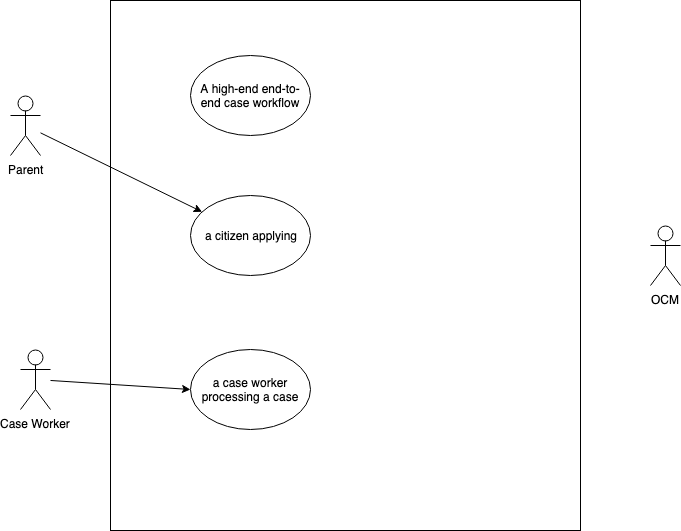
\includegraphics[width=\textwidth]{img/use-cases}
	\caption{Use case diagram}
\end{figure}

\newpage
\section{Detailed Use cases}

\subsection{UC01: A high-end end-to-end case workflow}

\begin{table}[htb!]
\begin{tabularx}{\textwidth}{l|X}
	\textbf{Use Case name} & A high-end end-to-end case workflow \\
	\hline
	\textbf{Participating actor} & Caseworker, User\\
	\hline
	\textbf{Flow of events} &
	\begin{compactenum}
			\item User creates application for loss of earnings,provides all needed information.
			\item Caseworker receives application, processes it and approves it.
			\item OCM sends email about the the approval of the application
			\item Calculation of compensation will be made by OCM
			\item OCM sets application on done
	\end{compactenum}\\
	\hline
	\textbf{Extensions} & 
	    \begin{compactenum}
	        \setcounter{enumi}{1}
	        \item \begin{compactenum}
	            \item Caseworker rejects application
	            \item OCM sends mail of rejection
	        \end{compactenum}
	    \end{compactenum}\\
	\hline
	\textbf{Entry condition} &
	Caseworker is logged in
	\\
	\hline
	\textbf{Exit condition} & 
	\begin{compactenum}
	    \item Caseworker is logged out
	\end{compactenum}
	\\
	\hline
	\textbf{Quality requirements} & See non-functional requirements in section \ref{sec:nfr}\\
\end{tabularx}
\end{table}

\subsection{UC02: A citizen applying}

\begin{table}[htb!]
\begin{tabularx}{\textwidth}{l|X}
	\textbf{Use Case name} & A citizen applying \\
	\hline
	\textbf{Participating actor} & User\\
	\hline
	\textbf{Flow of events} & 
	    \begin{compactenum}
	        \item User visits the portal
	        \item User initiates the process for applying loss of earnings
	        \item User fills out all the necessary information needed in the form
	        \item User uploads all required documentation
	        \item User uploads a doctor confirmation
	    \end{compactenum}\\
	\hline
	\textbf{Entry condition} & User is logged in\\
	\hline
	\textbf{Exit condition} & User saves the application and logs out\\
	\hline
	\textbf{Quality requirements} & See non-functional requirements in section \ref{sec:nfr}\\
\end{tabularx}
\end{table}

\subsection{UC03: A case worker processing a case}
\begin{table}[htb!]
\begin{tabularx}{\textwidth}{l|X}
	\textbf{Use Case name} & A case worker processing a case \\
	\hline
	\textbf{Participating actor} & Caseworker\\
	\hline
	\textbf{Flow of events} & 
	    \begin{compactenum}
	        \item Caseworker opens a newly opened application
	        \item Caseworker checks the documentation to be legitimate (including the provided doctor confirmation)
	        \item Caseworker approves application
	        \item OCM calculates 
	    \end{compactenum}\\
	\hline
	\textbf{Entry condition} & Caseworker is logged in\\
	\hline
	\textbf{Exit condition} & \\
	\hline
	\textbf{Quality requirements} & See non-functional requirements in section \ref{sec:nfr}\\
\end{tabularx}
\end{table}
% architecture model
\newpage
\section{Architecture model}
\begin{figure}[htb!]
    \centering
    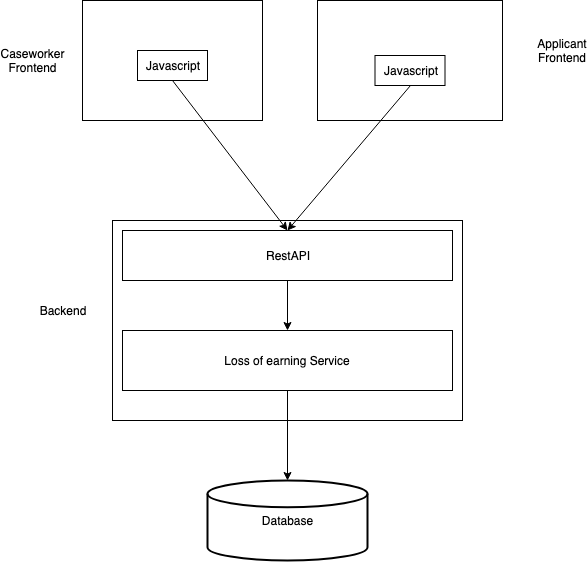
\includegraphics[width=\textwidth]{img/architecture-model.png}
    \caption{Architecture model}
\end{figure}

% project plan (shedule, work packages, skill matrix, risks)

\newpage
\section{Project plan}

\subsection{Team composition/roles}
\todo[inline]{Testing, UX etc.}
\textbf{Silvan Adrian}
\begin{itemize}
	\item SCRUM Master %otherwise won't make much sense of having a project team without a scrum master
\end{itemize}
\textbf{Matias Korn}
\begin{itemize}
	\item Developer
\end{itemize}
\textbf{Samuel Korn}
\begin{itemize}
	\item Developer
\end{itemize}
\textbf{Nikolin Prenga}
\begin{itemize}
	\item Developer
\end{itemize}

\subsection{Skill matrice}
\todo[inline]{extend skill matrice}
%fill up
\begin{table}[htb!]
\begin{tabular}{lllll}
 \textbf{Skill}  & \textbf{Silvan} & \textbf{Matias} & \textbf{Samuel} & \textbf{Nikolin} \\
\hline
Development       &                 &                   &                   &                  \\
Project Management &                 &                   &                   &                  \\
                  &                 &                   &                   &                 
\end{tabular}
\end{table}

\subsection{Work Packages}
% just a graph or actually some coding involved?

\subsection{Schedule}
As the project methodology SCRUM will be used, so after each Sprint there will be  working increment released.

\todo[inline]{(add more sprints, technically agile -> endless until it's done}
\begin{table}[htb!]
\begin{tabular}{lll}
\textbf{Sprint} & \textbf{Sprint Goal} & \textbf{Date} \\
\hline
1      & Set Up Infrastructure & xx.xx \\
2      & Do more etc.          &            \\
3       &                       &           
\end{tabular}
\end{table}

\subsection{Risks}
\todo[inline]{look into more Risks, technical as well}
\begin{table}[htb!]
\begin{tabularx}{\textwidth}{llllXX}
\textbf{Nr} & \textbf{Description} & \textbf{Probability} & \textbf{Criticality} & \textbf{Mitigation}                                                      & \textbf{Measure}                                                                             \\
\hline
R1          & Worker gets sick     & 10\%                 & high                 & Every worker should be able to replace the skill of an other in the team & Split up work not only according to someones skills but also to get them to learn new things \\
            &                      &                      &                      &                                                                          &                                                                                              \\
            &                      &                      &                      &                                                                          &                                                                                             
\end{tabularx}
\end{table}


\end{document}
